\documentclass{article}
\usepackage{stmaryrd}
\usepackage{graphicx}

\title{Report, Kinetic project}
\author{Dorian Geraldes Pereira, Axel Demuth}
\date{March 2024}

\begin{document}
\maketitle
\tableofcontents
\newpage
\section{Objectives}
the objective of the project is to process files in IFC format containing building meshes that are not hermetic in an algorithms repairing
geometric error in a kinetic data structures
\section{Tools}
\subsection{CGAL}
CGAL is a package for geometry algorithms,offering differents data structure and algorithms
to work on polygons,surface,mesh generation... 
\subsection{Kinetic}
Kinetic algorithms is a package from CGAL, he permit to work on mesh with some hole in it .
When applied on the mesh the Kinetic algorithms will 'prolonger' some surface to fill the mesh to make it 
waterproof.
we can see here what the algorithm is capable of :
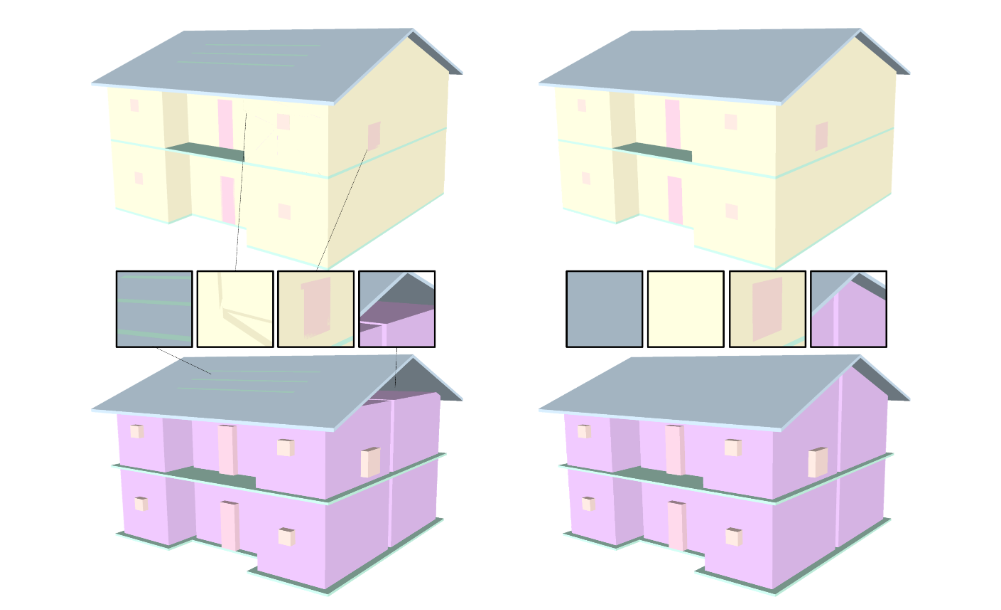
\includegraphics[scale =   0.3 ]{../../images/example_algorithm.png}
\nocite{*}
\bibliographystyle{plain}
\bibliography{../../bibliography/v0/report_bib}
\end{document}